% Knowledge Graphs Project - RC2526
% Updated D2 report in Springer LNCS format - simpler English, expanded slice section.
% Compile from this directory:
%   pdflatex kg_report_lncs && pdflatex kg_report_lncs
% Or from repo root:  bash submissions/compile.sh
\documentclass{llncs}
\usepackage[utf8]{inputenc}
\usepackage[T1]{fontenc}
\usepackage{microtype}
\usepackage{graphicx}
\usepackage{booktabs}
\usepackage{amsmath,amssymb}
\usepackage{tikz}
\usetikzlibrary{arrows.meta,positioning}

\begin{document}

\title{Link Prediction on FB15k-237:\\
Matched KGE Baselines and Self-Adversarial\\
Hard-Negative Sampling}

\author{Thalia Delhaise \and Lenny Briclet \and
        Andr\'e Fonseca \and Rafael Gufler}

\institute{RC2526, Knowledge Graphs (joint project with Deep Learning)}

\maketitle

% -----------------------------------------------------------------------
\begin{abstract}
We study \textbf{link prediction} on the \textbf{FB15k-237} benchmark
using two standard knowledge graph embedding models, \textsc{TransE} and
\textsc{RotatE}, trained under the \emph{same} conditions and evaluated
with the filtered ranking protocol.
Our 50-epoch baselines give RotatE MRR\,=\,0.261 and Hits@10\,=\,0.424
on the test set.
We now plan to extend training with \textbf{self-adversarial negative
sampling} from the RotatE paper, which makes the model focus on hard
examples rather than trivially easy ones.
The central question of our project is: \emph{do relation-level structural
patterns explain where RotatE beats TransE, and does hard-negative training
change those gaps?}
This report describes our method, our current results, and the experiments
we plan to run, and asks for feedback before we start coding.
\end{abstract}

% -----------------------------------------------------------------------
\section{Introduction and Motivation}

A \emph{knowledge graph} (KG) is a collection of facts stored as triples
$(h,r,t)$, where $h$ and $t$ are entities (e.g.\ \emph{Paris},
\emph{France}) and $r$ is the relation between them (e.g.\
\emph{capital\_of}).
\emph{Link prediction} is the task of completing a triple when one side is
hidden: given $(h,r,?)$ or $(?,r,t)$, which entity should fill the gap?
This is useful in many real-world settings, from question answering to
biomedical databases.

Training a link-prediction model requires \emph{negative examples}, i.e.\
fake triples that the model should score low.
Since we do not know all true facts, negatives are built by \emph{corrupting}
a real triple: take $(h,r,t)$ and replace $t$ with a random entity $t'$.
The problem is that most random replacements are \textbf{obviously wrong},
and once the model has learned the basics, it stops learning much from them.
\emph{Hard-negative sampling} solves this by choosing corruptions that
the model already finds \emph{plausible}, i.e.\ the cases where the
model is still making mistakes and needs more training signal.

Our project has three main contributions:
\begin{enumerate}
  \item \textbf{Matched baselines}: TransE and RotatE trained with the
        same setup, so their scores can be compared fairly.
  \item \textbf{Self-adversarial sampler}: a custom PyTorch module that
        selects hard negatives during training, compared against the
        standard random corruption.
  \item \textbf{Slice and error analysis}: breaking down the results by
        relation type and entity connectivity to understand \emph{where}
        each model does well or fails.
\end{enumerate}

\paragraph{Working hypothesis.}
Our main hypothesis is that self-adversarial negative sampling will not
improve all test cases uniformly.
Instead, we expect the largest gains to appear in the harder parts of the
graph, especially for low-frequency relations and low-degree entities,
where uniformly sampled negatives are often too easy to provide a useful
training signal.
The slice analysis is designed to test this hypothesis directly rather
than only reporting a single aggregate MRR score.

% -----------------------------------------------------------------------
\section{Problem, Data, and Evaluation}

\paragraph{Task.}
Given a knowledge graph $\mathcal{G}=(\mathcal{E},\mathcal{R},\mathcal{T})$
where $\mathcal{T}$ is the set of known triples, the goal is to rank all
candidate entities for a query $(h,r,?)$ or $(?,r,t)$ such that the
correct answer appears near the top.
The model is trained on $\mathcal{T}_{\text{train}}$; validation and test
sets contain disjoint held-out triples.

\paragraph{Dataset.}
We use \textbf{FB15k-237}, a standard benchmark derived from Freebase.
Inverse-relation pairs have been removed to avoid trivially easy predictions.
It contains 14,505 entities, 237 relation types, and
272,115\,/\,17,535\,/\,20,466 triples in train, validation, and test.
We compute graph statistics (relation frequencies, entity degrees) from
$\mathcal{T}_{\text{train}}$ only; using test data for those stats would
be a form of information leakage into our slice analysis.
Key numbers: mean entity degree $\approx$\,20, but the maximum in-degree
is 6,289, meaning the graph is very skewed: a few central entities appear
in thousands of triples while most appear in very few.
We load the official split using PyKEEN.

\paragraph{Evaluation.}
We use \textbf{filtered} MRR and Hits@$k$ ($k\in\{1,3,10\}$).
For each test query, we remove from the candidate list any entity that
would form a known true triple, so the model is not penalised for
correctly recalling a fact seen in training or validation.
We report the \emph{realistic} score (average of two tie-breaking
conventions) and average over head and tail queries (\texttt{both}).

% -----------------------------------------------------------------------
\section{Methodology}

\subsection{KGE Models: TransE and RotatE}

Both models learn a \emph{score} $f_\theta(h,r,t)\in\mathbb{R}$ for each
triple: true triples should get high scores and fake ones low scores.

\textbf{TransE} works in $\mathbb{R}^d$ and
defines the score as $f(h,r,t)=-\|h+r-t\|$: the idea is that adding the
relation vector to the head should land close to the tail.
This works well for simple, one-to-one relations but struggles with
symmetric or one-to-many ones.

\textbf{RotatE} uses complex-valued embeddings
($\mathbb{C}^d$) and models each relation as a rotation: $f(h,r,t)=-\|h
\circ r - t\|$ with $|r_k|=1$.
Because rotations can compose, invert, and repeat, RotatE can naturally
represent symmetric, inverse, and compositional relations, patterns that
are common in FB15k-237 and hard for TransE to capture.

\paragraph{Shared training setup.}
Both models are trained with \emph{identical} settings so their results
are directly comparable: embedding size $d=128$, Adam optimizer
(lr=$10^{-3}$), batch size 1024, up to 50 epochs, early stopping with
patience 10 on validation MRR, CUDA, and random seed 42 for the initial
baseline runs.
If compute allows, the final RotatE comparison will be repeated with
three seeds, $\{42,123,999\}$, and we will report mean and standard
deviation.
This makes the comparison more robust, since negative sampling methods can
be sensitive to random initialization and to the sampled corruptions.
We train both models with a shared Python pipeline and store all metrics,
curves, and model checkpoints in the project repository for reproducibility.

\subsection{Negative Sampling: Default vs.\ Self-Adversarial}
\label{sec:hard-neg}

\paragraph{Default Bernoulli corruption (current baseline).}
For each real triple $(h,r,t)$ we generate one fake triple by replacing
either the head or the tail with a random entity.
The choice of which side to corrupt follows the standard Bernoulli
heuristic: relations that tend to have many tails per head are more likely
to have their tail corrupted, while relations that tend to have many heads
per tail are more likely to have their head corrupted.
Crucially, this process does \emph{not} look at the model at all; the
same random replacements are sampled regardless of what the model has
learned so far.
As training progresses, many of these negatives become trivially easy and
therefore provide little gradient signal.

\paragraph{Self-adversarial hard-negative sampling (planned).}
We will implement the self-adversarial negative sampling strategy
introduced with RotatE.
Instead of training on a single random corruption, we first generate a pool
of $n$ candidate corruptions and then give higher weight to the candidates
that the current model scores as more plausible.
These are ``hard'' negatives: they are false triples, but the model is
currently close to treating them as true.

For computational reasons, we will use a fixed candidate pool size
$n=64$ in the main experiment.
If this is too expensive on GPU, we will fall back to $n=32$ and report
this choice explicitly.
We keep $n$ fixed during the main ablation so that the only tuned
hyperparameter is the self-adversarial temperature $\alpha$.

To avoid ambiguity in the sign convention, we define
$s_\theta(h,r,t)$ as the model score where \emph{higher means more
plausible}.
For distance-based models such as TransE and RotatE, this can be
implemented as a margin minus distance, e.g.
$s_\theta(h,r,t)=\gamma-d_\theta(h,r,t)$.

For a positive triple $(h,r,t)$, let
$\{(h,r,t'_i)\}_{i=1}^n$ be uniformly sampled tail corruptions, or
$\{(h'_i,r,t)\}_{i=1}^n$ uniformly sampled head corruptions, depending on
which side is corrupted.
For simplicity, the equations below show the tail corruption case.
Each negative receives the self-adversarial weight
\begin{equation}
  p_j
  =
  \frac{
    \exp\!\bigl(\alpha\, s_\theta(h,r,t'_j)\bigr)
  }{
    \sum_{i=1}^{n}
    \exp\!\bigl(\alpha\, s_\theta(h,r,t'_i)\bigr)
  },
  \label{eq:sadv}
\end{equation}
where $\alpha>0$ controls how strongly the distribution focuses on hard
negatives.

The training objective is then
\begin{equation}
  \mathcal{L}
  =
  -\log\sigma\!\bigl(s_\theta(h,r,t)\bigr)
  -
  \sum_{j=1}^{n}
  p_j\,
  \log\sigma\!\bigl(-s_\theta(h,r,t'_j)\bigr),
  \label{eq:loss}
\end{equation}
where $\sigma$ is the sigmoid.
The first term pushes the score of the true triple upward, while the
second term pushes the scores of the weighted negative triples downward.

\paragraph{Intuition.}
When $\alpha$ is small, the softmax in Eq.~\eqref{eq:sadv} is close to
uniform, so the method behaves similarly to random negative sampling.
As $\alpha$ increases, more probability mass is assigned to the negatives
with the highest model scores, i.e.\ those that the model currently finds
most confusing.
These examples are expected to provide a stronger training signal than
easy random corruptions.

However, very hard negatives are not always beneficial.
If $\alpha$ is too large, the model may over-focus on a small number of
highly scored corruptions, which can make training noisy or unstable.
For this reason, we will tune $\alpha\in\{0.5,1.0,2.0\}$ on the
validation set only and monitor both validation MRR and the training loss
curves.
The test set will only be used once for the final selected configuration.

\paragraph{Implementation plan.}
We will implement Eqs.~\eqref{eq:sadv} and~\eqref{eq:loss} in a standalone
PyTorch module, separate from the default PyKEEN training loop.
Training will reuse the same model architecture, data splits, optimizer,
batch size, evaluation protocol, and training budget as the baseline;
only the negative sampler changes.
This gives a clean ablation: any difference between the baseline RotatE
run and the self-adversarial RotatE run can be attributed mainly to the
negative sampling strategy.

We will record global metrics, per-slice metrics, training curves, and the
selected value of $\alpha$.
If compute allows, the final comparison will be repeated over three random
seeds to check whether the observed gains are stable.

\begin{figure}[t]
\centering
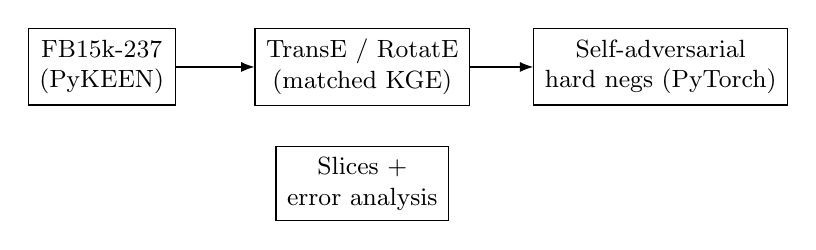
\begin{tikzpicture}[node distance=0.4cm, font=\small, >=Latex,
  box/.style={draw, align=center, inner sep=4pt}]
\node[box] (data) {FB15k-237\\(PyKEEN)};
\node[box, right=1.0cm of data] (kge) {TransE / RotatE\\(matched KGE)};
\node[box, right=0.8cm of kge] (neg)
      {Self-adversarial\\hard negs (PyTorch)};
\node[box, below=0.5cm of kge] (slice) {Slices +\\error analysis};
\path[->] (data) edge (kge) (kge) edge (neg);
\path[->] (kge.south) -- (slice.north);
\end{tikzpicture}
\caption{Project pipeline. The self-adversarial sampler replaces
the default Bernoulli corruption, while the evaluation code stays
identical so the comparison is fair.}
\label{fig:pipeline}
\end{figure}

% -----------------------------------------------------------------------
\section{Baseline Results}

Table~\ref{tab:baseline} shows test-set scores for both models after
50 epochs with default Bernoulli negatives (no hard-negative sampling).
Early stopping never triggered: the best checkpoints were at epoch\,45
for TransE and epoch\,44 for RotatE, meaning both models were still
improving at the end of training.

\begin{table}[t]
\centering
\caption{Test-set filtered metrics, realistic ranking, \texttt{both}
  (head and tail averaged).
  Training: 50\,ep max, patience\,10, $d$=128,
  Adam lr=$10^{-3}$, bs=1024, CUDA, seed=42, default Bernoulli negatives.}
\label{tab:baseline}
\begin{tabular}{@{}lcccccc@{}}
\toprule
Model   & MRR   & H@1   & H@3   & H@10  & H@10 head & H@10 tail \\
\midrule
TransE  & 0.152 & 0.073 & 0.174 & 0.304 & 0.201 & 0.407 \\
RotatE  & \textbf{0.261} & \textbf{0.179} & \textbf{0.286} &
          \textbf{0.424} & \textbf{0.312} & \textbf{0.536} \\
\bottomrule
\end{tabular}
\end{table}

RotatE outperforms TransE on every metric under the same training
conditions: MRR goes from 0.152 to 0.261 ($+72\%$) and H@10 from
0.304 to 0.424 ($+39\%$).
One striking observation is the gap between head and tail prediction for
RotatE: H@10 is 0.312 for head queries but 0.536 for tail queries.
This means the model is much better at predicting ``who is connected to
this entity via this relation'' than at predicting ``which entity connects
to this target''.
This asymmetry suggests that different types of relations behave very
differently, which motivates the slice analysis in Section~\ref{sec:plan}.

\begin{figure}[t]
\centering
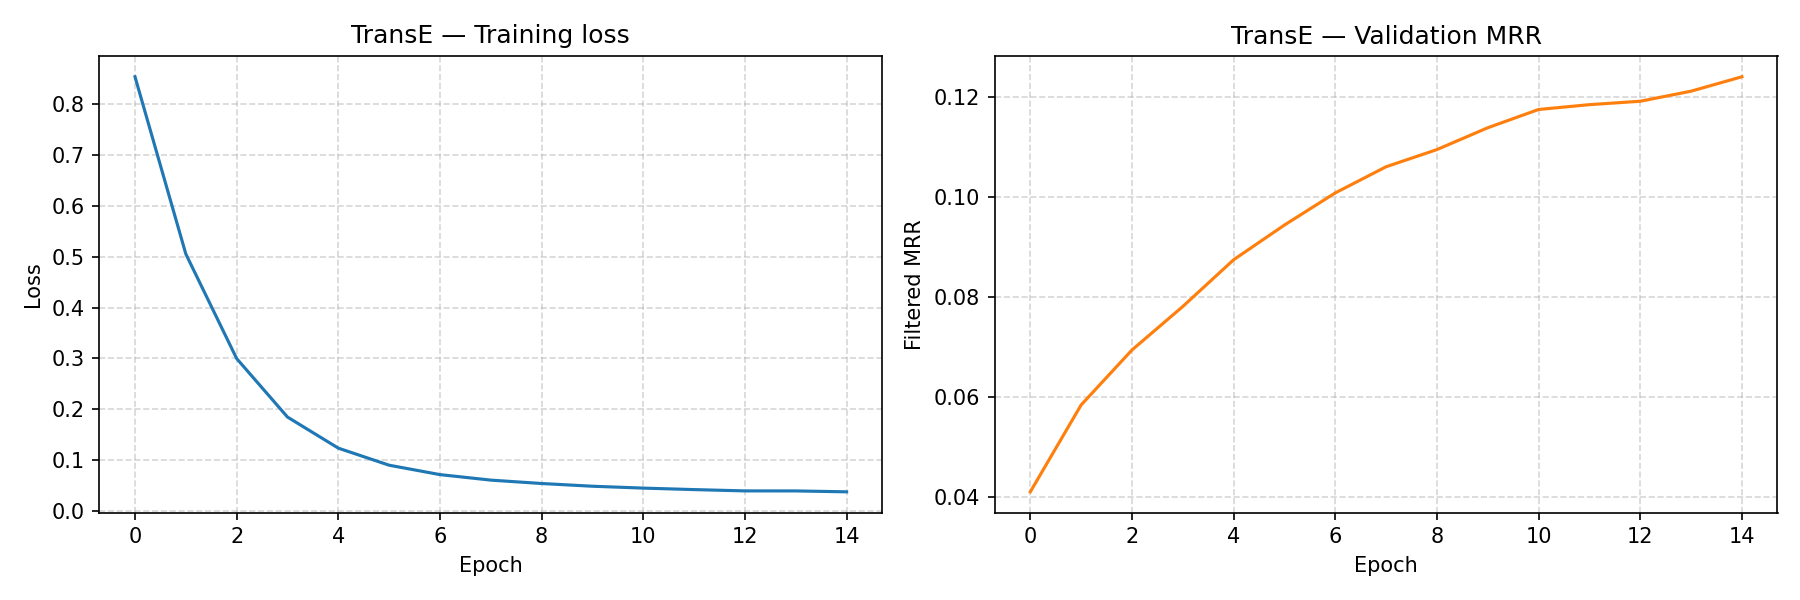
\includegraphics[width=0.48\linewidth]{../../../artifacts/baseline/TransE_curves.png}
\hfill
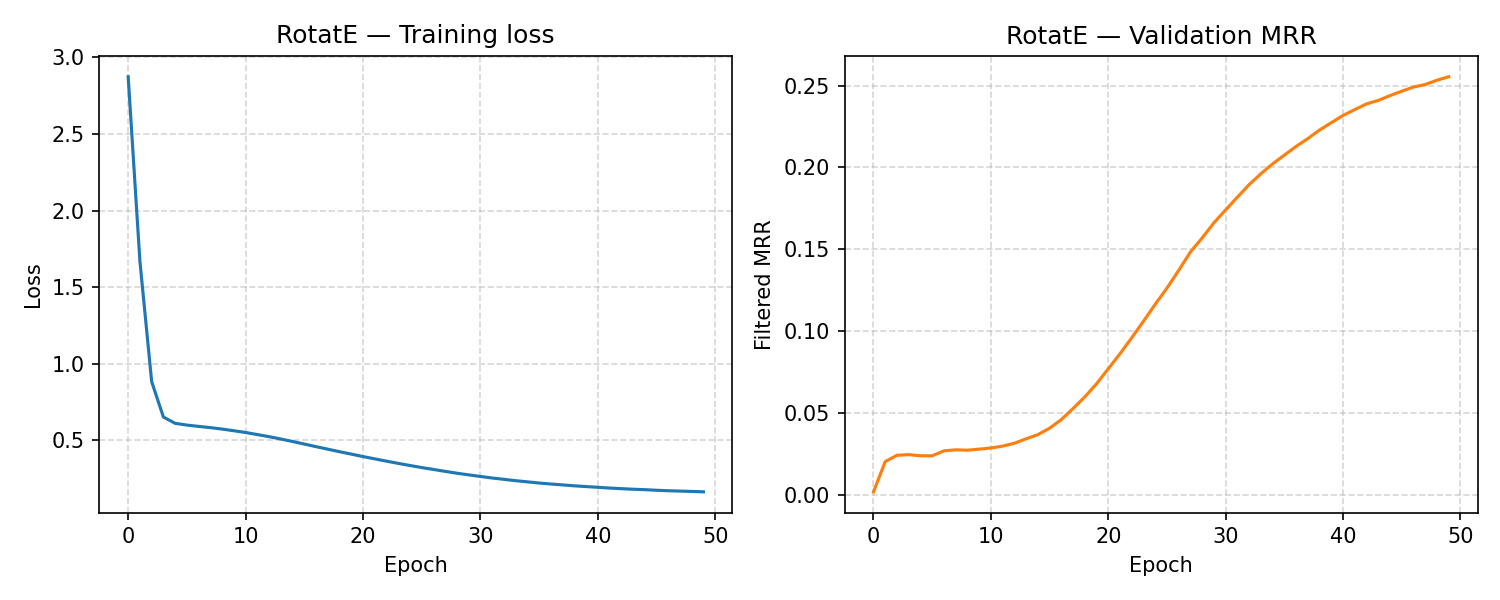
\includegraphics[width=0.48\linewidth]{../../../artifacts/baseline/RotatE_curves.png}
\caption{Training loss and validation MRR over 50 epochs for TransE
  (left) and RotatE (right), default Bernoulli negatives, CUDA.
  Validation MRR is still rising at epoch 50 for both models.}
\label{fig:curves}
\end{figure}

% -----------------------------------------------------------------------
\section{Planned Experiments}
\label{sec:plan}

\paragraph{Ablation: default vs.\ self-adversarial negatives.}
The main experiment keeps everything fixed and changes \emph{only} the
negative sampling strategy:
(a) default Bernoulli negative sampling, already used in
Table~\ref{tab:baseline}, versus
(b) self-adversarial negative sampling with $\alpha$ selected on the
validation set.
The model architecture, embedding dimension, optimizer, batch size,
training budget, data splits, and filtered evaluation protocol remain
unchanged.

We will run this ablation at minimum on \textbf{RotatE}, since it is the
stronger baseline and the method was introduced in the RotatE paper.
If time allows, we will also run the same comparison on TransE to test
whether the sampler helps only RotatE or whether the effect is more
general.
The expected outcome is an additional row in Table~\ref{tab:baseline}
labelled ``RotatE + self-adv.'', together with a discussion of whether the
gain is global or concentrated in specific relation/entity slices.

If compute allows, the final RotatE baseline and RotatE+self-adversarial
configuration will be repeated with seeds $\{42,123,999\}$.
Otherwise, we will clearly report that the comparison is based on a single
seed and treat the result as indicative rather than definitive.

\paragraph{Slice evaluation.}
\label{sec:slices}

The global MRR numbers in Table~\ref{tab:baseline} summarise performance
across all 20,466 test triples at once.
But FB15k-237 is not uniform: some relations appear thousands of times in
training while others appear only a handful of times, and some entities
are connected to thousands of others while most are not.
A single aggregate score hides whether the model is good across the board
or only on the easy, frequent cases.

\emph{Slice evaluation} addresses this by splitting the test triples into
groups, called \textbf{slices}, and computing MRR and H@10
\emph{separately within each group}.
This lets us ask more precise questions, such as: does RotatE's advantage
over TransE hold equally for rare relations and for frequent ones?
Does hard-negative training help more for entities with many connections
or for isolated ones?

Concretely, we plan two types of slices:

\begin{enumerate}
  \item \textbf{Relation-frequency slices.}
    We count how often each relation appears in $\mathcal{T}_{\text{train}}$
    and divide the 237 relations into four frequency bins (quartiles).
    Test triples are then assigned to a bin based on their relation.
    A relation that appears 15,000 times in training is a ``high-frequency''
    relation; one that appears only 50 times is ``low-frequency''.
    We expect models to do better on high-frequency relations because they
    have seen more examples of them.
    The interesting question is whether self-adversarial negatives help
    \emph{more} on low-frequency relations, where random negatives are
    especially uninformative.

  \item \textbf{Entity-degree slices.}
    We compute the number of triples in $\mathcal{T}_{\text{train}}$ that
    involve each entity, i.e.\ its degree, and again split into four bins.
    High-degree entities, for example a country that appears in thousands
    of triples, are ``easy'' in the sense that the model has seen them in
    many contexts.
    Low-degree entities, for example a minor person appearing in just a few
    triples, are harder because the model has little evidence about them.
    We will report scores separately for queries involving high-degree vs.\
    low-degree entities, to see whether hard negatives close the gap.
\end{enumerate}

Crucially, all statistics, including relation frequencies and entity
degrees, are computed from $\mathcal{T}_{\text{train}}$ only.
Using test-set statistics to define the slices would leak information
about the test distribution into our analysis.

We will report per-slice MRR and H@10 for TransE default, RotatE default,
and RotatE self-adversarial, so the table directly shows where each model
gains and where hard negatives help most.

In addition to relation-frequency and entity-degree slices, we will also
report head-query versus tail-query performance, since the baseline results
already show a strong asymmetry.
This extra slice is cheap to compute and helps determine whether
self-adversarial negatives mainly improve head prediction, tail prediction,
or both.

\paragraph{Error analysis.}
To complement the numbers, we will inspect a small set of concrete
examples.
For a few representative relations, chosen to cover different frequency
levels and structural types, for example symmetric or compositional
relations, we will look at cases where RotatE ranks the correct entity in
the top\,10 but TransE does not, and at cases where both models fail.
These examples will help illustrate the slice results and give an
intuition for what kinds of mistakes each model makes.

\paragraph{Optional: relational GNN.}
A shallow R-GCN trained on the same
splits is a possible extension if the above experiments are complete
before the final deadline.
It is not the main focus of the project.

% -----------------------------------------------------------------------
\section{Discussion and Request for Feedback}

The self-adversarial sampler described in Section~\ref{sec:hard-neg} is
our main new contribution beyond using PyKEEN out of the box.
We chose it for three reasons: (i)~it comes directly from the RotatE
paper, so it is well motivated for our main model; (ii)~it can be
implemented as a small standalone PyTorch module without changing the
model architecture; and (iii)~because we already have the baseline runs,
the ablation is straightforward to set up.

The main risk is that hard negatives are not guaranteed to improve all
cases.
If the adversarial distribution becomes too sharp, training may over-focus
on a small number of confusing corruptions.
For this reason, we keep the candidate pool size fixed, tune only
$\alpha$ on validation, and monitor both validation MRR and training
stability.

\medskip\noindent
\textbf{We would welcome feedback on the following points before we start
implementing:}
\begin{itemize}
  \item Is self-adversarial negative sampling, as described in
        Equations~\ref{eq:sadv} and~\ref{eq:loss}, an appropriate main
        extension for the scope of this project, or would a simpler or
        higher-level alternative be more suitable?
  \item Is the ablation design sound, i.e.\ keeping the model, optimizer,
        training budget, and evaluation protocol fixed while changing only
        the negative sampler?
  \item Is fixing the candidate pool size to $n=64$ and tuning only
        $\alpha\in\{0.5,1.0,2.0\}$ on validation a reasonable compromise
        between experimental control and computational cost?
  \item Is the slice analysis based on relation frequency, entity degree,
        and head-query versus tail-query performance sufficient to support
        our main claim about where hard negatives help?
  \item Would you recommend repeating the final comparison with multiple
        seeds, or is a single-seed comparison acceptable for the scope of
        this project?
\end{itemize}

\end{document}